\section{Mitosis-Core}
Mitosis-Core implements the algorithm of the Peer-to-Peer mesh network that is presented in \vref{chap:design}. The main task is to connect peers and to set up an overlay network. To make it use-case agnostic and extendable it offers the core functionality through a slim interface.

The source code in \vref{lst:mitosis-api} demonstrates how the interface can be used.
The basic functionality that is provided, is listening on entering or leaving peers (\cref{line:MitObserverPeerChurn}), sending a message to a discovered peer (\cref{line:sendMessage}) and to listen on incoming messages (\cref{line:MitObserverInbox}).

\begin{Listing}[htb!]
\begin{lstlisting}[basicstyle=\tiny,basicstyle=\footnotesize\ttfamily,xleftmargin=3em]
const mitosis = new Mitosis();

mitosis.getPeerManager()
  .observePeerChurn() |\label{line:MitObserverPeerChurn}|
  .subscribe(ev => {
    const peerId = ev.peer.getId();
    if (ev.type === ChurnType.ADDED) {
      mitosis.sendMessageTo(peerId, 'Hello!'); |\label{line:sendMessage}|
      console.log(`Peer ${peerId} entered`);
    } else if (ev.type === ChurnType.REMOVED) {
      console.log(`Peer ${peerId} left`);
    }
  });
  
mitosis.getInbox() |\label{line:MitObserverInbox}|
  .subscribe(message => {
    console.log(message.getBody());
  });
\end{lstlisting}
\caption{Basic usage of Mitosis}
\label{lst:mitosis-api}
\end{Listing}

Mitosis-Core also allows the configuration of some internal parameters that are used by the algorithm like connection goals or signal server address. In case the default configuration does not fit the use-case, the application can overwrite the default values with custom settings.

\subsection{Mitosis-Core Architecture}
Mitosis-Core consists of several components. Before they are further explained, \vref{fig:mit-core-architecture} presents the overall architecture to give a glimpse of the inner workings.

\begin{sidewaysfigure}
\centering
\vspace{15cm}
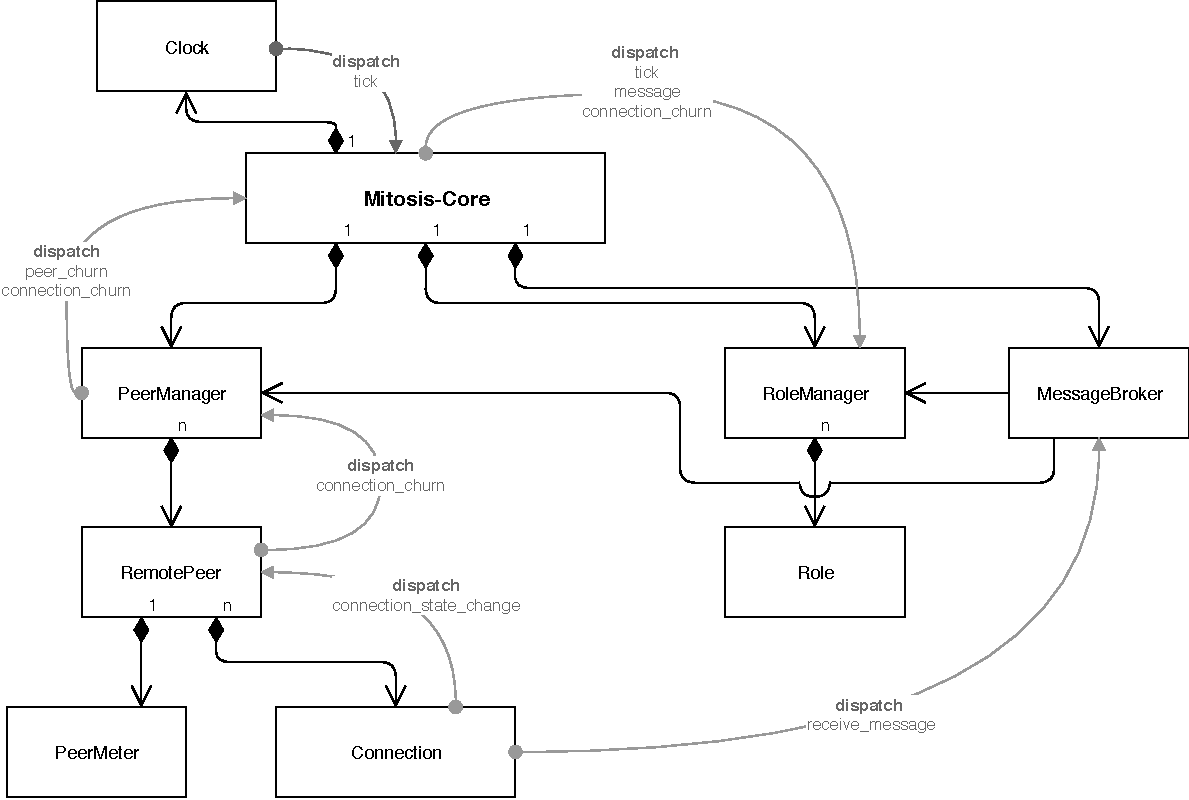
\includegraphics[width=0.9\textwidth]{graphics/implementation/mitosis-architecture.pdf}
\caption{Mitosis-Core components}
\label{fig:mit-core-architecture}
\end{sidewaysfigure}
